\documentclass[UTF8, a4paper]{ctexart}
\usepackage[margin=1in]{geometry} % 页边距调整
\usepackage{ctex}
\usepackage{array, amsmath, amssymb}

\usepackage{booktabs, tabularx, multirow, multicol} % 表格拓展支持
\usepackage{graphicx, subfigure, float} % 图片排版支持

\usepackage{algorithm, algpseudocode} % 伪代码支持
\renewcommand{\algorithmicrequire}{\textbf{Input:}}  
\renewcommand{\algorithmicensure}{\textbf{Output:}} 

\usepackage{tikz, mathpazo} % 基本绘图支持
\usepackage{flowchart} % 流程图支持
\usepackage{pgf-umlcd} % UML类图支持
\usetikzlibrary{arrows, shapes, chains, shapes.geometric}

\usepackage{listings} % 代码块支持
\usepackage{xcolor}
\lstset{
	language		= c++,
	backgroundcolor	= \color{white},
	basicstyle		= \footnotesize\ttfamily,
	keywordstyle	= \color{blue},
	stringstyle		= \color{red!58!blue!82}\ttfamily,
	commentstyle	= \color{darkgray},
	rulesepcolor	= \color{red!20!green!20!blue!20},
	columns			= fullflexible,
	breaklines		= true,
	captionpos		= b,
	tabsize			= 4,
	frame			= single,
	escapeinside	= {\%*}{*)}
}
%%示例
% \begin{lstlisting}[caption={}]
% #include <iostream>
% int main(int argc, char *argv[]) {
% 	std::cout << "Hello World!" << std::endl;
% 	return 0;
% }
% \end{lstlisting}

\usepackage{datetime} %日期
\renewcommand{\today}{\number\year{年}\number\month{月}\number\day{日}}

\begin{document}

\begin{center}
	\zihao{3}《数据结构》实验报告
\end{center}
\zihao{5}

\newcolumntype{Y}{>{\raggedleft\arraybackslash}X}
\noindent\begin{tabularx}{\textwidth}{XcY}
	  {班 级:}\;\underline{DL062123}
	& {姓 名:}\;\underline{项乔栋}
	& {学 号:}\;\underline{2021302468} \\
	  {邮 箱:}\;\underline{13282135976@sina.cn}
	& {日 期:}\;\underline{\today}
	& {编 号:}\;\underline{DS03}
\end{tabularx}
~\\

\noindent\textbf{$\circledcirc$
实验题目:\quad{稀疏矩阵转置}} \par
\noindent\textbf{$\circledcirc$
实验目的:\quad{实践密集矩阵方法到稀疏矩阵的迁移}} \par
\noindent\textbf{$\circledcirc$
实验内容:\quad{基于三元组的稀疏矩阵转置实现}} \par

\subsection*{一、需求分析}
\noindent\fbox{
\begin{tabularx}{\textwidth}{lY}
\bf{Description}
& \parbox[t]{\linewidth}{
	输出稀疏矩阵的转置矩阵。(行列均不大于20)
} \\

\bf{Input}
& \parbox[t]{\linewidth}{
	第一行输入两个正整数n和m,分别表示矩阵的行数和列数,然后输入矩阵三元组,最后输入(0 0 0)表示结束输入。
} \\

\bf{Output}
& \parbox[t]{\linewidth}{
	转置后的矩阵
} \\

\bf{Sample Input}
& \fbox{\parbox[t]{\linewidth}{\bf{
	\mbox{4 4} \\
	\mbox{1 1 1} \\
	\mbox{2 1 2} \\
	\mbox{3 2 3} \\
	\mbox{0 0 0}
}}} \\

\bf{Sample Output}
& \fbox{\parbox[t]{\linewidth}{\bf{
	\mbox{1 1 1} \\
	\mbox{1 2 2} \\
	\mbox{2 3 3}
}}}
\end{tabularx}}

\subsection*{二、概要设计}
为保持基于三元组的稀疏矩阵的有序性并兼顾算法效率,使用统计方法预处理稀疏矩阵,得到相关信息,以直接定位转置后元素的位置。 \par
1.\;基本操作: \par
	CreateFromIO() $\rightarrow$ SparseMatrix \par
	\qquad\textbf{操作结果:}\;从IO流创建稀疏矩阵 \par
	Tranpose(matrix:SparseMatrix) $\rightarrow$ SparseMatrix \par
	\qquad\textbf{操作结果:}\;获取转置稀疏矩阵 \par
	Output(matrix:SparseMatrix) $\rightarrow$ void \par
	\qquad\textbf{操作结果:}\;输出稀疏矩阵 \par
2.\;程序模块: \par
1) 主程序 \par
2) IO支持 \par
3) 稀疏矩阵转置 \par
\begin{figure}[H]
	\begin{minipage}[t]{\linewidth}
		\centering
		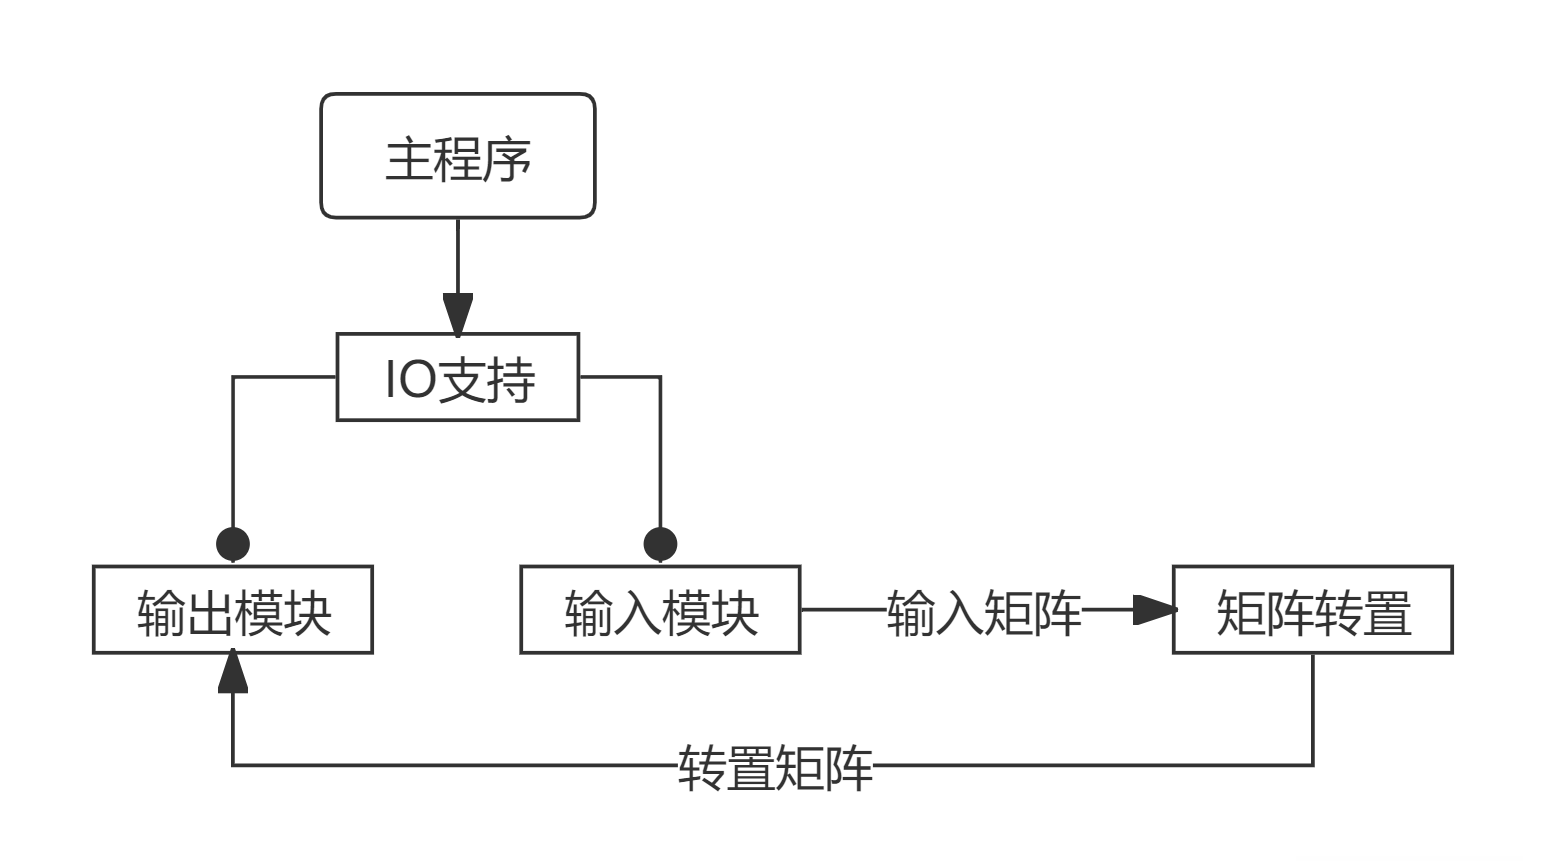
\includegraphics[width=125mm,height=64mm]{./assets/DS03-1}
	\end{minipage}
\end{figure}

\subsection*{三、详细设计}
\begin{algorithm}
\begin{algorithmic}[1]
\caption{Sparse Matrix Transpose based on Triple}
\Require SparseMatrix: $\mathbf{matrix}$
\Ensure $\mathbf{matrix}^T$
\State let $\mathbf{transposed}$ $\leftarrow$ SparseMatrix\{ size=$\mathbf{matrix}$.size() \}
\State let $\{P_i\}$ $\leftarrow$ \{start position of column i in transposed matrix\}
\For {e in $\mathbf{matrix}$}
	\State let t $\leftarrow$ \{ e.column, e.row, e.value \}
	\State $\mathbf{transposed}[P_{t.row}]$=t
	\State $P_{t.row}$=$P_{t.row}$+1
\EndFor
\State return $\mathbf{transposed}$
\end{algorithmic}
\end{algorithm}

\subsection*{四、使用说明、测试分析与结果}
\subsubsection*{1、使用说明}
1) 本程序可以通过任意编译器生成目标文件并在当前平台运行。 \par
2) 进入程序后依照需求的输入样式输入数据,手动输入与流式输入都是被允许的。特别的是,在你的数组长度不大于1024的情况下,当前给出的实验程序并不强制要求输入数组长度不大于20。 \par
3) 请确保输入矩阵的行列标从0开始计数。 \par
4) 鉴于具体算法实现,避免输入过大的矩阵(如$2^{30}$×$2^{30}$的规模),以防内存分配失败导致程序崩溃。
\subsubsection*{2、测试结果与分析}
2.1\;\textbf{实际环境} \par
对于所有输入,矩阵元素以行主序输入;对于大部分输入,矩阵规模远大于非零元素规模 \par
2.2\;\textbf{边界情况} \par
无 \par
2.3\;\textbf{测试结果} \par
目标代码通过全部测试,无需纠正
\subsubsection*{3、调试过程问题分析与解决办法}
原代码提交NOJ产生了RE反馈,故断言是数组越界问题。经过分析判定原代码在预设情境下逻辑完备,故怀疑是NOJ的数据问题。通过对数组下标检查并手动中止算法过程,破坏算法完整性,从而顺利地获得了WA的反馈。故而问题与预期一致,是预设情景与NOJ实际输入存在偏差。在我的预设情境下,输入矩阵的行列标从1计数,而实际输入的行列标从0计数,故而整体移动下标,解决问题。
\subsubsection*{4、设计与实现的回顾讨论与分析}
转置后的矩阵以原列主序存储,若能够统计各列的元素个数,就能够得到各列在转置矩阵中的首元素位置。使用该数据进行的转置元素插入可以在常数时间完成,为了保证算法的有效性,只需维护各列首元素位置数据。使用该算法达成目标的一个缺点是,首元素位置的维护往往需要占用大量内存空间,不过通常该损失是可以接受的。
\subsubsection*{5、运行界面}
\begin{figure}[H]
	\begin{minipage}[t]{\linewidth}
		\centering
		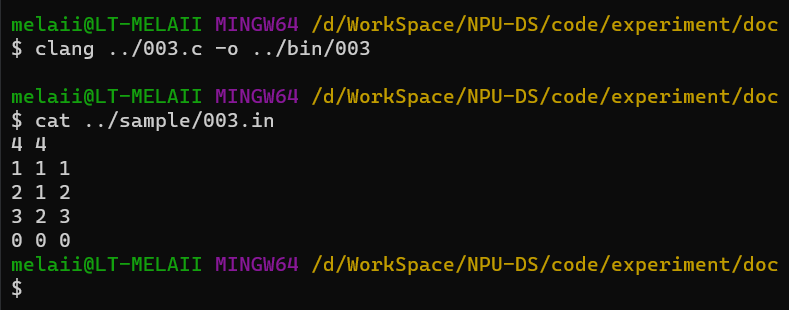
\includegraphics[width=125mm,height=50mm]{./assets/DS03-2}
		\caption{前置环境}
	\end{minipage}
\end{figure}
\begin{figure}[H]
	\begin{minipage}[t]{\linewidth}
		\centering
		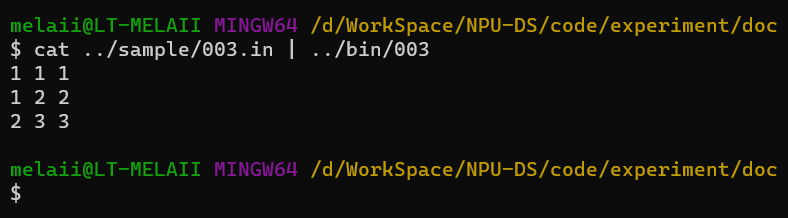
\includegraphics[width=125mm,height=40mm]{./assets/DS03-3}
		\caption{结果输出}
	\end{minipage}
\end{figure}

\subsection*{五、实验总结}
对于三元组实现的稀疏矩阵,它的有序性不是天然的,需要手动维护。该实验存在多种有效的完成途径:(1)暴力查找插入(2)翻转+排序(3)统计定位插入。本文提供的算法完成的是途径(3),不难发现,在完成统计后,该算法的插入是常数的。但是当矩阵过于稀疏时,预处理的开销将超过转置本身的操作并且消耗大量内存,此时则采取途径(2)更为适合。该实验与常规矩阵存储形式的转置虽然表现相同,但是内核却不尽相同。常规形式进行行和列的拷贝呼唤,而三元组稀疏矩阵的转置则侧重在维护有序性上,它的转置操作反而是微不足道的。这大概便是使用的数据结构的不同带来的解决问题的思路不同。

~\\
\zihao{-4}
\textbf{教师评语:}
~\\
\textbf{实验成绩:}

\begin{flushright}
\mbox{指导教师签名:\qquad\qquad} \\
\mbox{批阅日期:\qquad\qquad}
\end{flushright}

\end{document}